\chapter{Experiment}


\begin{figure}
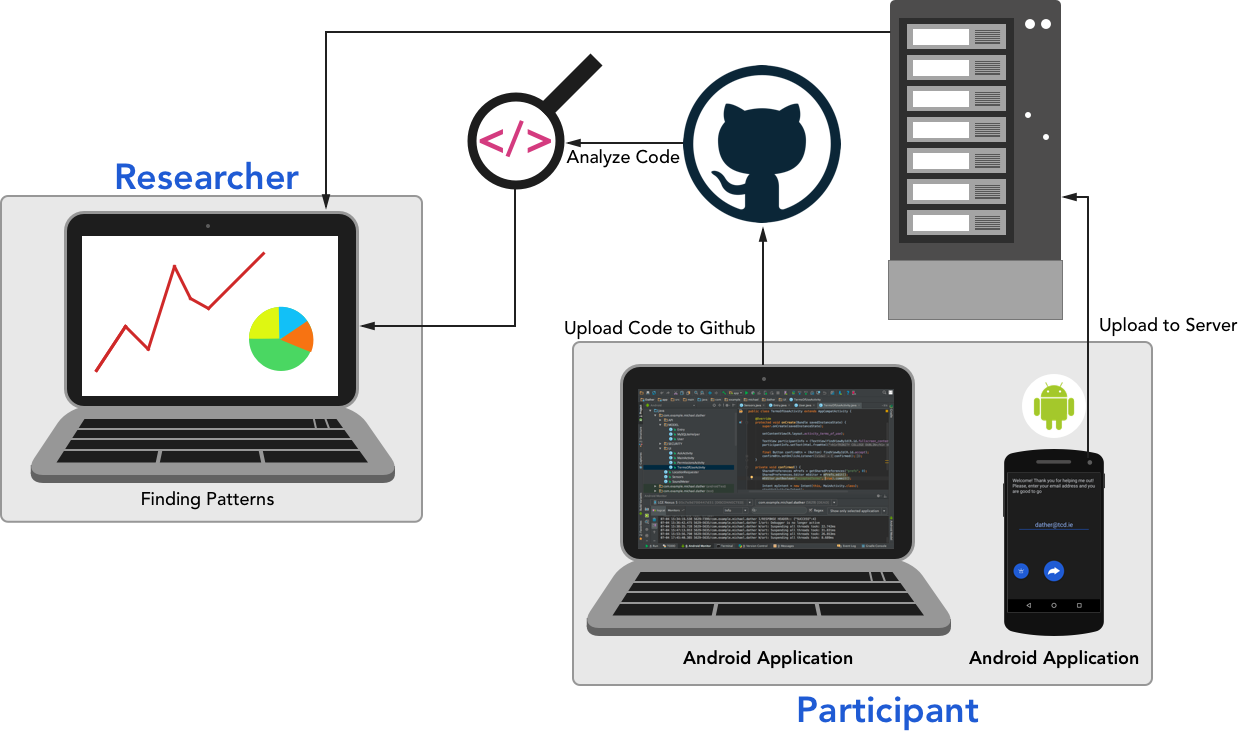
\includegraphics[width=\textwidth]{experiment}
\caption{Experiment Execution}\label{experiment}
\vspace{10 mm}
\end{figure}

In the experiment, participants are solving a programming task while the Dather Android App is running to record behavior and environmental factors. After the submitted code is been analyzed, its been compared with the gathered data in order to find correlations between the participants performance and the information from the gathered data. You can see the flow of the experiment in Figure \ref{result}. 
\section{Setup and Execution}
Every participants need to have access to a mobile phone with Android version 4.4 or later. In order to participate at the experiment the participants need to install the Dather Application of the device. The Application can be downloaded from the website \url{http://frickm.de} when it's been accessed from the Android device. 
After installing the downloaded apk-file, the participants permits the application to gather the data and allows the data to be used for research. 
The last step before being able to start the experiment, the user needs to enter his/her email address.\\
After setting up the application and accessing the website with a programming task, the experiment is ready to start. The participant starts the gathering process while working on the programming task.\\
After completing the task, the participant uploads the solution code to Github and sends a link of the Github repository from the Email address which was entered in the Android application. 

\section{Expected Results}
Based on the previous work of other researchers in this area and based on my own experience, I expect to find correlations between the code quality and the environmental noise. The high amount of distraction noises will probably negatively influence the concentration of the participants and decrease the code quality. My own experience showed me that background music can improve the cognitive functionality but depending on the concentration which is needed for the task. Before doing research I was sure to find correlations between sunshine and a better performance compared to cloudy or even rainy days for a big amount of the participants. Anyways, I think that the result might show different groups of people that perform different in the same environment compared to each other. It would be possible to find out that some group of people work better at night listening to music and another group performs best during the morning on a bench in a quite park.
